\documentclass[a4paper,titlepage,11pt]{ltjsarticle}
\usepackage[dvipdfmx]{graphicx}
\usepackage{color}
\usepackage{amssymb}
\usepackage{here}
\usepackage{subcaption}
\usepackage{amsmath}
\usepackage{listings}
\lstset{
	%プログラム言語(複数の言語に対応,C,C++も可)
	language = Java,
	%背景色と透過度
	backgroundcolor={\color[gray]{.90}},
	%枠外に行った時の自動改行
	breaklines = true,
	%自動改行後のインデント量(デフォルトでは20[pt])	
	breakindent = 10pt,
	%標準の書体
	basicstyle = \ttfamily\scriptsize,
	%コメントの書体
	commentstyle = {\itshape \color[cmyk]{1,0.4,1,0}},
	%関数名等の色の設定
	classoffset = 0,
	%キーワード(int, ifなど)の書体
	keywordstyle = {\bfseries \color[cmyk]{0,1,0,0}},
	%表示する文字の書体
	stringstyle = {\ttfamily \color[rgb]{0,0,1}},
	%枠 "t"は上に線を記載, "T"は上に二重線を記載
 %他オプション:leftline,topline,bottomline,lines,single,shadowbox
	frame = TBrl,
	%frameまでの間隔(行番号とプログラムの間)
	framesep = 5pt,
	%行番号の位置
	numbers = left,
 %行番号の間隔
	stepnumber = 1,
 %行番号の書体
	numberstyle = \tiny,
 %タブの大きさ
	tabsize = 4,
	%キャプションの場所("tb"ならば上下両方に記載)
	captionpos = t
}
%目次を付け加える。
\setcounter{secnumdepth}{5}
\renewcommand{\lstlistingname}{}
\begin{document}

\title{情報システム工学実験Ⅱ \\後半フルレポート}
\author{2022531033 関川謙人}
\date{\today}
\maketitle
% 目次の出力
\tableofcontents
\clearpage
\section{背景}
\subsection{経緯}
元々関数電卓や数字パズルゲームを作ることを画策していたのだが電卓は数式の表示方法
やデザイン性を考えたときにいい物が思いつかなかった。またパズルゲームはデザインや
ゲーム性に独創性を見いだせずアイデアに行き詰まる。

一旦諦めて友人と話していた時に東方
の話になり、高校時代に東方風神録をプレイしていたことを思い出した。そこでZUN氏の
アイデアを借りて東〇風シューティングゲームを制作することを思いつき、制作するに至った。
\subsection{制作目的}
本アプリの制作目的は以下のとおりである。
\begin{itemize}
	\item 知っているシューティングゲームの挙動を一通り実装できるようになる。
	\item ゲーム制作の基礎を体感し、ゲームプログラミングの基礎を理解する。
	\item 試行錯誤を行うことでゲームクリエイターの創造性を理解する。
\end{itemize}
\subsection{本実験の目的}
Processingという一つのツールを使えるようになり、自身の独創性を発揮する手段
として用いる。このことで新しい開発プラットフォームを使いこなせるようにする学習能力を身に着ける
ことが本実験の目的である。
\section{実験方法}
\subsection{実験装置}
本実験における実験や開発は、VisualStudioCode(以下VSCode)上で行った。
拡張機能は以下のものを入れている。
\begin{itemize}
	\item Processing VSCode
	\item Processing Formatter
\end{itemize}
Processing VSCodeにProcessingの実行ファイル、Processing.javaを実行させる。
こうすることで図\ref{inventry}のようにVSCode上でコーデング、ファイル実行が
行える環境を構築できる。

またProcessing FormatterでProcessingコードの整形を行った。

自機や敵機の画像はclip studio paintで制作した。
%開発環境の画像%
\begin{figure}[H]
	\begin{center}
		\includegraphics*[height = 8cm]{invent_view.png}
		\caption{開発環境}
		\label{inventry}
	\end{center}
\end{figure}
\subsection{開発計画}
開発の手順を計画段階と実際の手順とで比べると、以下の表のようになる。
\begin{table}[H]
\begin{center}
	\footnotesize
	\begin{tabular}{|p{48truemm}|p{48truemm}|} \hline
		計画段階 & 実際の開発 \\
	\hline \hline
		%箇条書き
		\begin{minipage}{48truemm}
			\begin{enumerate}
				\setlength{\leftskip}{-8truemm}
				\item 自機を定義
				\item 敵機を定義
				\item 通常攻撃を定義
				\item 必殺技を定義
				\item 当たり判定を定義
				\item 各種パラメータを定義
			\end{enumerate}
		\end{minipage}
			 &
		\begin{minipage}{48truemm} %ここで列の幅が決まります
			\begin{enumerate}
				\setlength{\leftskip}{-7truemm}
				\item 自機の動作を定義
				\item 自機の攻撃を定義
				\item 敵機の当たり判定を定義
				\item 敵機の動作を定義
				\item 敵機の攻撃を定義
				\item 自機の当たり判定を定義
				\item 自機、敵機のパラメータを定義
				\item 5,6を繰り返す
				\item 自機、敵機のグラフィックを定義
				\item ボム(自機の必殺技)を定義
				\item フェーズ、ゲーム終了等のシステム面を定義
				\item 歯車型の敵を定義。
				\item 5,6を行い、最終フェーズを構築
			\end{enumerate}
		\end{minipage}
	\\	\hline
	\end{tabular}
\end{center}
\end{table}
\section{アプリの概要}
\label{app_detail}
このゲームのコンセプトは敵の弾を避けながらプレイヤーの
必殺技を駆使して敵を倒すことにある。
この章では、完成したアプリについて以下の観点から説明する。
\begin{itemize}
	\item システム・仕様
	\item 自機の動作
	\item 敵機の動作
\end{itemize}
また各処理の実装に用いたソースコードを一部省略して掲載している。
\subsection{システム・仕様}
\ref{app_detail}節を説明するのに使う用語の定義は以下の通り。
\begin{table}[H]
	\begin{center}
		\begin{tabular}{|c|c|}
			\hline
			用語 & 定義 \\ \hline \hline 
			自機 & プレイヤーが操作するオブジェクト \\ \hline
			敵 & 後述するEnemyクラスで定義されるオブジェクト全般 \\ \hline
			敵機 & プレイヤーの討伐目標。 \\ \hline
			必殺技 & 敵の弾幕あるいはプレイヤーの攻撃手段\\ \hline
			フェーズ & ゲームのプレイ段階 \\ \hline
		\end{tabular}
	\end{center}
\end{table}
このゲームの仕様は以下のとおりである。
\begin{itemize}
	\item 実行した際、スタート画面が表示される。
	\item スタート画面にてcキーでゲームスタート
	\item 敵機のHPが0になったら勝ち
	\item 自機のHPが0になったら負け
	\item 敵の攻撃は4通り存在する
	\item 敵の攻撃の種類は敵の残りHPによって決まる
	\item 勝敗が決まると終了判定画面に移行する。
	\item 終了判定画面にてeキーでゲーム終了、cキーでもう一度プレイする
	\item もう一度プレイする際、すべての変数がリセットされる。
\end{itemize}
%横に2枚の画像(jpg/png)表示
\begin{figure}[H]
\begin{center}
\begin{tabular}{c}
\begin{minipage}{0.3\hsize}
\begin{center}
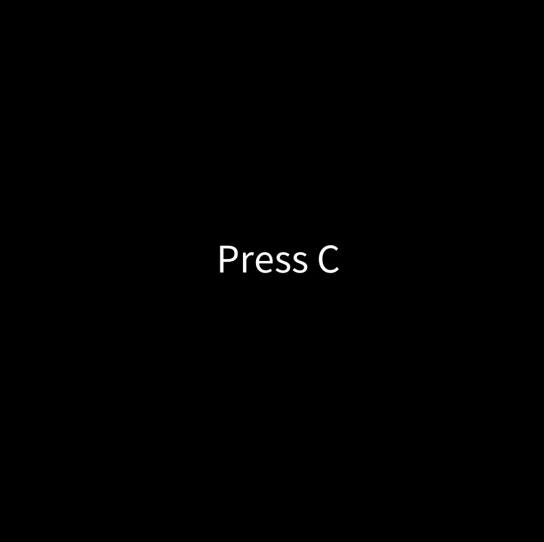
\includegraphics[width=3.5cm]{start.png}
\end{center}
\caption{スタート画面}
\label{start}
\end{minipage}
\begin{minipage}{0.3\hsize}
\begin{center}
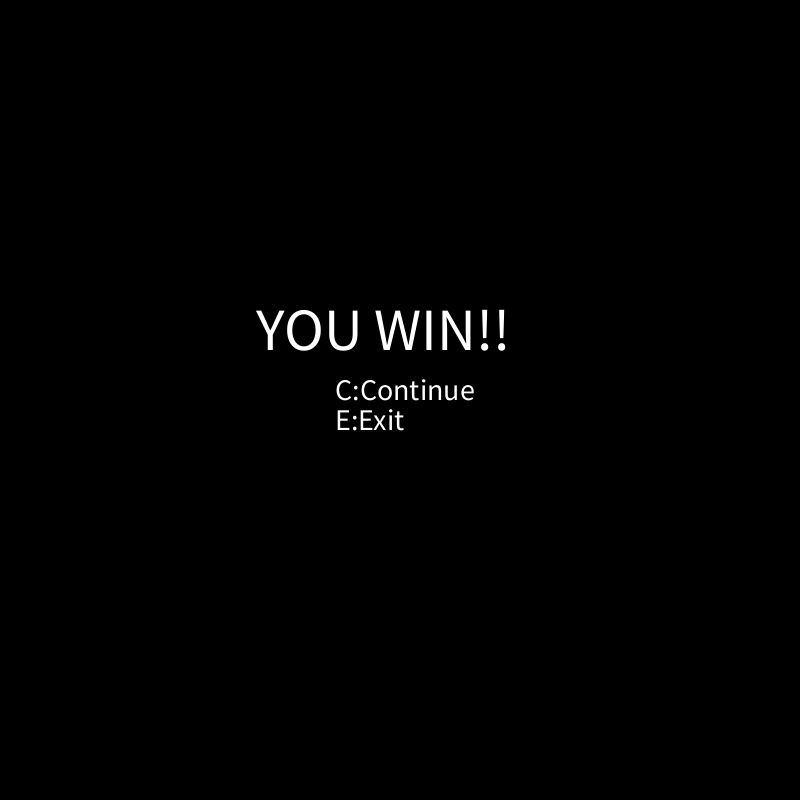
\includegraphics[width=3.5cm]{drawing_30.png}
\end{center}
\caption{終了判定画面(勝利時)}
\label{judge_end}
\end{minipage}
\end{tabular}
\end{center}
\end{figure}

\subsubsection{使用した変数・関数}
システムの構築に使用した変数は以下のとおりである
\begin{table}[H]
	\begin{center}
		\begin{tabular}{|c|c|c|}
			\hline
			型 & 変数・関数 & 説明 \\ \hline \hline
			int & Game\_width & ゲーム画面の横幅。512に設定。 \\ \hline
			int & phase & フェーズを表す変数  \\ \hline
			int & frameCount & フレーム数 \\ \hline
			boolean & game\_play & ゲームプレイ画面かどうか \\ \hline
			boolean & ckey & cキーが押されているかどうか  \\ \hline
			boolean & ekey & eキーが押されているかどうか \\ \hline
			void & status() & ステータス画面を表示する関数 \\ \hline
			void & judge() & 勝敗の判定を行い、結果を表示する関数 \\ \hline
			void & continue\_judge() & 継続判定を行う関数 \\ \hline
			void & judge\_phase() & 敵のHPを基にフェーズ判定を行う関数 \\ \hline
		\end{tabular}
	\end{center}
\end{table}
\subsubsection{ソースコード}
システム面は以下のソースコードで管理している。敵機や自機、必殺技に
関連する変数が含まれているがそれに関しては後述の節で説明する。
\begin{lstlisting}
void setup(){
	//ウィンドウサイズ(800*800)
	size(800,800);
}
void draw() {
  background(0); //画面の初期化

  //スタート画面
  if (phase == 0) {
      color(255);
      textSize(60);
      text("Press C" , width / 2 - 80, height / 2);
      //Cキーを押してスタート
      if (ckey) {
          phase = 1;
      }
  }
  if (game_play && phase > 0) {
      status();
        judge_phase(); //フェーズ管理
	}
	judge();
  if (!game_play) {
      continue_judge();
  }
	frameCount++;
}
	//ゲーム状況を表示
void status() {
    strokeWeight(3);
    stroke(0,0,400);
    fill(0,0,400);
    line(Game_width + 2,0,Game_width + 2,height);
    textSize(60);
    text("YOU",Game_width + 60, height * 3 / 4); 
    text("Enemy",Game_width + 60,height / 4);
    image(shiratuyu_head, width - 120, height * 3 / 4 - 40 ,40,40);
    textSize(40);
    text("HP:" + player.HP + " / " + player.Max_HP, Game_width + 30 , height * 3 / 4 + 60);
    text("XP:" + player.XP + "/" + player.Max_XP, Game_width + 30 , height * 3 / 4 + 100);
    textSize(30);
    text("HP:" + enemy.HP + "/" + enemy.Max_HP , Game_width + 30, height / 4 + 60);
    text("phase : " + phase , Game_width + 30, height / 4 + 90);
    image(murasame_head, width - 50 , height / 4 - 30,40,40);
}
//勝敗の判定
void judge() {
    textSize(60);
    fill(0,0,400);
    if (enemy.HP <= 0) {
        text("YOU WIN!!",Game_width / 2, height / 2 - 50);
        game_play = false;
    }
    else if (player.HP <= 0) {
        text("GAME OVER",Game_width / 2, height / 2 - 50);
        game_play = false;
    }
}
//継続判定
void continue_judge() {
    if (game_play == false) {
        textSize(30);
        text("C:Continue",width / 2 - 65, height / 2);
        text("E:Exit",width / 2 - 65, height / 2 + 30);
        if (keyPressed) {
            if (ckey) {
                //初期化して再開
                game_play = true;
                player.x = Game_width / 2;
                player.y = height - 100;
                enemy.x = Game_width / 2;
                enemy.y = height / 4;
                player.HP = player.Max_HP;
                player.XP = player.Max_XP;
                enemy.HP = enemy.Max_HP;
                if (NumOfBullet > 0) {
                    for (int i = NumOfBullet - 1; i >= 0; i--) {
                        bullets.remove(i);
                    }
                }
                if (NumOfBullet2 > 0) {
                    for (int i = NumOfBullet2 - 1; i >= 0; i--) {
                        bullet2.remove(i);
                    }
                }
                if (NumOfRect > 0) {
                    for (int i = NumOfRect - 1; i >= 0; i--) {
                        Rect_attack.remove(i);
                    }
                }
                if (NumOfCParts > 0) {
                    for (int i = NumOfCParts - 1; i >= 0; i--) {
                        Cparts.remove(i);
                    }
                }
                if (NumOfsinb > 0) {
                    for (int i = NumOfsinb - 1; i >= 0; i--) {
                        sinb.remove(i);
                    }
                }
                if (NumOfcosb > 0) {
                    for (int i = NumOfcosb - 1; i >= 0; i--) {
                        cosb.remove(i);
                    }
                }
                if(NumOfgear > 0){
                    for(int i = NumOfgear - 1; i >= 0; i--){
                        gear.remove(i);
                    }
                }
                if(NumOfgearb > 0){
                    for(int i = NumOfgearb - 1; i >= 0; i--){
                        gear_bullet.remove(i);
                    }
                }
                NumOfBullet = 0;
                NumOfBullet2 = 0;
                NumOfRect = 0;
                NumOfCParts = 0;
                NumOfsinb = 0;
                NumOfcosb = 0;
                NumOfbomb = 0;
                NumOfgear = 0;
                NumOfgearb = 0;
                gear_push = true;
                usebullet = 0;
                frameCount = 0;
                phase = 1;
            }
            if (ekey) {
                exit();
            }
        }
    }
}
void judge_phase() {
    if (phase != 0) {
        if (enemy.HP > enemy.Max_HP * 11 / 13) {
            phase = 1;
        }
        else if (enemy.HP > enemy.Max_HP * 7 / 13) {
            phase = 2;
        }
        else if (enemy.HP > enemy.Max_HP * 3 / 13) {
            phase = 3;
        }
        else if (enemy.HP <= enemy.Max_HP * 3 / 13) {
            phase = 4;
        } 
    }
}
\end{lstlisting}
\subsubsection{処理の説明}
背景色は黒、ウィンドウサイズは縦800、横800である。
status()関数では画面をゲームプレイ画面とステータス画面に分割する。
そしてステータス画面に以下を表示する。
\begin{itemize}
	\item 敵機のHP
	\item フェーズ
	\item 自機のHP
	\item 自機のXP
\end{itemize}

judge()関数では敵機、自機どちらのHPが0であるかを判定する。自機のHP
が0であれば"GAME OVER"と表示し、敵機のHPが0であれば"YOU WIN!!"と表示する。

仕様をわかりやすく示したのが以下の図である。
\begin{figure}[H]
\begin{center}
\includegraphics*[height = 8cm]{playing_phase1.png}
\caption{プレイ画面}
\end{center}
\end{figure}

judge\_phase()関数で制御されるフェーズの移行条件は以下の表のとおりである
\begin{table}[H]
	\centering
	\begin{tabular}{|c|c|}
		\hline
		フェーズ & 移行条件\\ \hline \hline
		0 & スタート画面 \\ \hline
		1 & スタート画面または終了判定画面でcを押す \\ \hline
		2 & 敵のHPが最大HPの11/13\\ \hline
		3 & 敵のHPが最大HPの7/13 \\ \hline
		4 & 敵のHPが最大HPの3/13 \\ \hline
	\end{tabular}
\end{table}
各フェーズの説明については\ref{Enemy}項で細かく説明する。
\subsubsection{必殺技の基本定義}
必殺技の定義ついてもここで説明する。定義にはWeaponクラスを使用している。

全ての必殺技はArrayList<Weapon>という形で定義している。
これによってWeaponクラスを基にしたオブジェクトの動的配列で
必殺技を制御できる。以下の表はこのプログラムに使用したArrayListのコマンドの一覧である
\begin{table}[H]
	\begin{center}
		\begin{tabular}{|c|c|}
			\hline
			コマンド & 説明 \\ \hline \hline
			object = ArrayList.<class> & オブジェクトの動的配列の定義 \\ \hline
			object.add & オブジェクトを追加 \\ \hline
			object.remove(i) & i番目のオブジェクトを削除 \\ \hline
			object.get(i) & i番目のオブジェクトを参照 \\ \hline
		\end{tabular}
	\end{center}
\end{table}
\paragraph{使用した関数・変数}

Weaponクラス内のフィールド(変数)は以下の表のとおりである。
\begin{table}[H]
	\begin{center}
		\begin{tabular}{|c|c|c|}
			\hline
			型 & 変数・関数 & 説明 \\ \hline \hline
			class & Weapon & 必殺技を定義するクラス \\ \hline
			float & x & 弾のx座標 \\ \hline
			float & y & 弾のy座標 \\ \hline
			float & speed & 弾の速度 \\ \hline
			float & atk & 弾の攻撃力 \\ \hline
			float & vecX & 弾のx進行方向 \\ \hline
			float & vecY & 弾のy進行方向 \\ \hline
		\end{tabular}
	\end{center}
\end{table}

\paragraph{ソースコード}
以下に、Weaponクラスを定義するソースコードを示す。

\begin{lstlisting}[caption={ソースコード\ref{Weapon}}]
	class Weapon{
    //フィールドの宣言
    float x;
    float y;
    float speed;
    float atk;
    float XP;
    float vecX;
    float vecY;
    //Weaponクラスのコンストラクタ
    Weapon(float xpos ,float ypos,float sped, float attack,float XP,float vecX,float vecY) {
        x = xpos;
        y = ypos;
        speed = sped;
        atk = attack;
        this.XP = XP;
        this.vecX = cos(radians(vecX));
        this.vecY = sin(radians(vecY));
    }
}
\end{lstlisting}
\label{Weapon}
以降、Weaponクラス内のフィールド、コンストラクタの記述は省略する。
\subsection{自機の動作}
この項目では自機の動作とプログラムについて
\begin{enumerate}
	\item 自機の基本動作
	\item 自機の基本技
	\item ボム
\end{enumerate}
の三つの観点から説明する。
\subsubsection{自機の基本動作}
\paragraph{使用した関数・変数}
自機の基本動作を定義する際使用した変数は以下の表のとおり。
\begin{table}[H]
		\label{player_funk}
		\centering
		\caption{プレイヤー定義に使用した変数}
		\begin{tabular}{|c|c|c|}
			\hline
			型 & 変数・関数 & 説明\\ \hline \hline
			class & Player\{\} & 自機を定義するクラス \\ \hline		
			Player & player & プレイヤーを表すオブジェクト \\ \hline	
			float & x & プレイヤーのx座標 \\ \hline
			float & y & プレイヤーのy座標 \\ \hline
			float & speed & プレーヤーの移動速度 \\ \hline
			float & HP & プレイヤーのHP \\ \hline
			float & Max\_HP & プレイヤーの最大HP \\ \hline
			float & XP & プレイヤーのXP。ボムの項目でも説明する。 \\ \hline
			float & Max\_XP & プレイヤーの最大XP \\ \hline
			boolean & is\_up & 上移動するかどうか\\ \hline
			boolean & is\_down &  下移動するかどうか\\ \hline 
			boolean & is\_right & 右移動するかどうか \\ \hline
			boolean & is\_left & 左移動するかどうか \\ \hline
			float & speed & プレイヤーの移動スピード \\ \hline
			void & movement() & プレイヤーの移動を制御\\ \hline
			void & display() & プレイヤーを表示する関数 \\ \hline
			なし & shiratuyu & 自機の画像 \\ \hline
		\end{tabular}
\end{table}

\paragraph{パラメータ}
自機のパラメータを以下の表に示す。
\begin{table}[H]
	\centering
	\begin{tabular}{|c|c|}
		\hline
		パラメータ & 値 \\ \hline \hline
		初期x座標 & Game\_width / 2 \\ \hline
		初期y座標 & height / 3 \\ \hline
		スピード(通常移動) & 5\\ \hline
		スピード(低速移動) & 2 \\ \hline 
		最大HP & 350 \\ \hline
		最大XP & 70 \\ \hline
	\end{tabular}
\end{table}
\paragraph{ソースコード}
以下に、プレイヤーの動作定義に使ったソースコードを示す。
%% ソースコード %%
\begin{lstlisting}
	void setup(){
		shiratuyu = loadImage("shiratuyu_dot.png");
		//クラス定義
    player = new Player(Game_width / 2,height / 3,false,false,false,false,5,350,350,70,70); //playerの初期化。
    //Player(x初期値,y初期値,上キー,下キー,右キー,左キー,プレイヤースピード,HP,Max_HP,XP,Max_XP)
	}
	//繰り返し処理。
void draw() {
    if (game_play && phase > 0) {
        player.display(); //プレイヤー表示
        player.movement(); //プレイヤーを動かす。 
    }
}
	void keyPressed() {
    //プレイヤーの動作
    if (key == CODED) {
        if (keyCode == UP) {
            player.is_up = true;
        }
        if (keyCode == DOWN) {
            player.is_down = true;
        }
        if (keyCode == RIGHT) {
            player.is_right = true;
        }
        if (keyCode == LEFT) {
            player.is_left = true;
        }
        if (keyCode == SHIFT) {
            player.speed = 2;
        }
    }
}

// キーを離したとき
void keyReleased() {
    //プレイヤーの動作
    if (key == CODED) {
        if (keyCode == UP) {
            player.is_up = false;
        }
        if (keyCode == DOWN) {
            player.is_down = false;
        }
        if (keyCode == RIGHT) {
            player.is_right = false;
        }
        if (keyCode == LEFT) {
            player.is_left = false;
        }
        if (keyCode == SHIFT) {
            player.speed = 5;
        }
    }
}
class Player{
	//フィールドの宣言
	//プレイヤー表示
	//プレイヤーの座標。
	float x;
	float y;
	//十字キーが押されているかの判定
	boolean is_up;
	boolean is_down;
	boolean is_right;
	boolean is_left;
	//---------------
	boolean movable = true;
	float speed; //プレイヤーの移動スピードを定義。
	float HP;
	float Max_HP;
	float XP;
	float Max_XP;
	//コンストラクタを宣言
	Player(float position_x,float position_y,boolean up,boolean down,boolean right,boolean left,float speed_arg , float health , float Max_HP,float XP, float Max_XP) {
			x = position_x;
			y = position_y;
			is_up = up;
			is_down = down;
			is_right = right;
			is_left = left;
			speed = speed_arg;
			HP = health;
	}
	// Playerクラス内で使用する関数
	void display() {
			noStroke();
			image(shiratuyu,x - 50,y - 55);
	}
	// プレイヤーを動かす。
	void movement() {
			if (y > 0 && is_up) {
					y -= speed;
					//-----敵に当たった時-----//
					if (dist(x,y,enemy.x,enemy.y) < 40) {
							y += speed;
							player.HP -= 1;
					}
			}
			if (y <= height && is_down) {
					y += speed;
					//----敵に当たった時-----//
					if (dist(x,y,enemy.x,enemy.y) < 40) {
							y -= speed;
							player.HP -= 1;
					}
			}
			if (x <= Game_width && is_right) {
					x += speed;
					//-----敵に当たった時-----//
					if (dist(x,y,enemy.x,enemy.y) < 40) {
							x -= speed;
							player.HP -= 1;
					}
			}
			if (x >= 0 && is_left) {
					x -= speed;
					//-----敵に当たった時-----//
					if (dist(x,y,enemy.x,enemy.y) < 40) {
							x += speed;
							player.HP -= 1;
					}
			}
	}
}
\end{lstlisting}
\paragraph{処理の説明}

キー入力があり、かつプレイヤーが枠内に収まっているときプレイヤーは1フレームにつき5ずつ動く。

敵座標との距離が40以内であるときプレイヤーは1ダメージを受ける。
敵機のいる方向に移動しようとすると以下の図のように
逆方向に動かされる。これによって敵にぶつかる処理を実装している。
%画像%
\begin{figure}[H]
	\begin{center}
		\includegraphics*[height = 5cm]{enemy_reject.png}
		\caption{敵との衝突処理}
	\end{center}
\end{figure}

SHIFTキーで低速移動を行う。
\subsubsection{自機の基本技}
プレイヤーがzキーを押したとき弾が発射できるようになっている。この弾を自機弾、
自機弾を発射する必殺技を基本技と定義する。
\begin{figure}[H]
\begin{center}
\includegraphics*[height = 6cm]{basic_avility.png}
\caption{基本技}
\end{center}
\end{figure}

\paragraph{使用した関数・変数}
新たに使用した関数・変数は以下の表のとおり
\begin{table}[H]
	\begin{center}
		\begin{tabular}{|c|c|c|}
			\hline 
		 型・クラス & 変数・関数 & 説明\\ \hline \hline
		 ArrayList<Weapon> & bullets & 左側の自機弾 \\ \hline
		 ArrayList<Weapon> & bullets2 & 右側の自機弾 \\ \hline
		 int & NumOfBullet & 左側の自機弾の数 \\ \hline
		 int & NumOfBullet2 & 右側の自機弾の数 \\ \hline
		 boolean & z\_push & zキーが押されているかどうか \\ \hline
		 void & movebullet() & 自機弾を上に動かす関数 \\ \hline
		 void & control\_bullet() & 自機弾の管理 \\ \hline
		 float & dist() & 二点間の距離を算出する組み込み関数 \\ \hline 
		\end{tabular}
	\end{center}
\end{table}

\paragraph{パラメータ}
自機弾のパラメータを表で示すと以下の通りになる。
\begin{table}[H]
\centering
\begin{tabular}{|c|c|}
	\hline
	パラメータ & 説明 \\\hline \hline
	初期x座標 & プレイヤーのx座標-10(bullet),+10(bullet2) \\ \hline
	初期y座標 & プレイヤーのy座標-22 \\ \hline
	弾速 & 20 \\ \hline 
	攻撃力 & 10 \\ \hline
	進行方向 & 上(y負方向) \\ \hline
\end{tabular}
\end{table}

\paragraph{ソースコード}
%システム面の場所に移動するのもあり。
以下に基本技を定義するソースコードを示す。
\begin{lstlisting}
void setup(){
	bullets = new ArrayList<Weapon>(); //味方の弾を定義
	bullet2 = new ArrayList<Weapon>(); //味方の弾(二個目)を定義
}
void draw(){
	if (game_play && phase > 0) {
      //Zキーを押して弾を発射
      if (z_push) {
          if ((player.speed == 5 && frameCount % 5 == 0) || (player.speed == 2 && frameCount % 2 == 0)) {
              bullets.add(new Weapon(player.x - 10,player.y - 22,20,10,0,0,0));//弾の生成
              bullet2.add(new Weapon(player.x + 10,player.y - 22,20,10,0,0,0));//弾の生成
              //弾の数のカウントを増やす
              NumOfBullet++;
              NumOfBullet2++;
      }
      //Weapon(初期x座標,初期y座標,弾速,攻撃力,消費XP,x進行方向,y進行方向)
      control_bullet();
  	}
	}
}

// キーを押したとき
void keyPressed() {
    if (key == 'z' || key == 'Z') {
        z_push = false;
    }
}
// キーを離したとき
void keyReleased() {
	if (key == 'z' || key == 'Z'){
		z_push = false
	}
}
class Weapon{
	// 球を動かす
    void movebullet() {
        fill(0,0,400);
        noStroke();
        y -= speed;
        ellipse(x,y,10,10);
    }
}
//自機弾の制御
void control_bullet() {
    for (int i = 0; i < NumOfBullet - 1; i++) {
        bullets.get(i).movebullet();
        //画面外に出たとき、要素を削除する。
        if (bullets.get(i).y < 0) {
            bullets.remove(i);
            NumOfBullet--;
        }
        //敵の当たり判定。敵に当たった時ダメージを与え、弾を消去する。
       if ((bullets.get(i).x < enemy.x + 30 && bullets.get(i).x > enemy.x - 30) && (bullets.get(i).y > enemy.y - 30 && bullets.get(i).y < enemy.y + 30)) {
            enemy.HP -= bullets.get(i).atk;
            bullets.remove(i);
            NumOfBullet--;
        }
    }
    //自機弾(2個目)の制御
    for (int i = 0; i < NumOfBullet2 - 1; i++) {
        bullet2.get(i).movebullet();
        //画面外に出たとき、要素を削除する。
        if (bullet2.get(i).y < 0) {
            bullet2.remove(i);
            NumOfBullet2--;
        }
        //当たり判定
        if ((bullet2.get(i).x < enemy.x + 30 && bullet2.get(i).x > enemy.x - 30) && (bullet2.get(i).y > enemy.y - 30 && bullet2.get(i).y < enemy.y + 30)) {
            enemy.HP -= bullet2.get(i).atk;
            bullet2.remove(i);
            NumOfBullet2--;
        }
    }
}
\end{lstlisting}

\paragraph{処理の説明}
zキーが押されている間、以下の挙動を行う。
\begin{itemize}
	\item プレイヤーのスピードが5(通常移動)の時5フレーム間隔で弾を発射する。
	\item プレイヤーのスピードが2(低速移動)の時2フレーム間隔で弾を発射する。
\end{itemize}
movebullet()関数では1フレーム毎に弾を上に動かす。弾速20であるため20ずつ
動かしている。※図\ref{move_bullet}

control\_bullet()関数では以下の役割を果たしている。
\begin{enumerate}
	\item 弾が範囲外に出たとき弾を消去する
	\item 敵の当たり判定に当たった時敵にダメージを与え、弾を消去する。
\end{enumerate}

自機弾については図\ref{control_bullet}のように敵の上下左右30を敵の当たり判定としている。
また弾が一つ当たるたびに敵に10ダメージを与える。

%横に2枚の画像(jpg/png)表示
\begin{figure}[H]
\begin{center}
\begin{tabular}{c}
\begin{minipage}{0.5\hsize}
\begin{center}
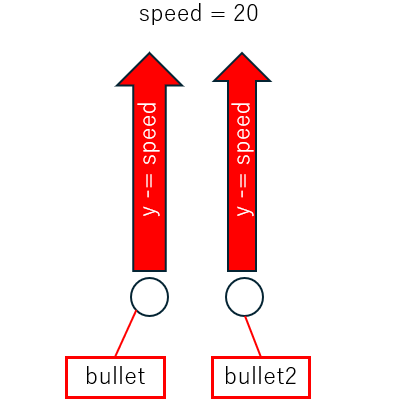
\includegraphics[width=8cm]{move_bullet.png}
\end{center}
\caption{弾が上に動く仕組み}
\label{move_bullet}
\end{minipage}
\begin{minipage}{0.5\hsize}
\begin{center}
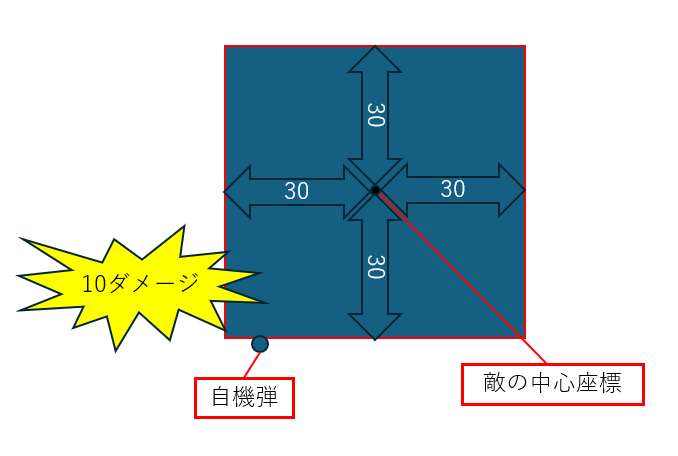
\includegraphics[width=8cm]{control_bullet.png}
\end{center}
\caption{弾の当たり判定}
\label{control_bullet}
\end{minipage}
\end{tabular}
\end{center}
\end{figure}
\subsubsection{ボム}
ボムには以下の特徴がある
\begin{itemize}
	\item xキーで発射できる
	\item ランダムな位置に発生
	\item 円状である
	\item 時間経過に応じて半径が大きくなる ※図\ref{bomb_larger}
	\item 半径が200を超えたとき消滅する
	\item 一度に8個発動できる
	\item 半径内の弾を消す。※図\ref{bomb_enemy}
	\item 半径内の敵にダメージを与える。※図\ref{bomb_enemy}
\end{itemize}
\begin{figure}[H]
\begin{center}
\includegraphics*[height = 8cm]{bomb_game.png}
\caption{}
\end{center}
\end{figure}

\paragraph{使用した変数・関数}
ボムの定義には新たに以下の変数・関数を使用した。
\begin{table}[H]
	\centering
	\begin{tabular}{|c|c|c|}
		\hline
		型・クラス & 変数・関数 & 説明\\ \hline \hline
		ArrayList<Weapon> & bomb & ボムのオブジェクト \\ \hline
		int & x\_count & xボタンを押してからの時間経過 \\ \hline
		int & NumOfbomb & ボムの数 \\ \hline
		float & r & ボムの半径 \\ \hline
		float & distance & ボムとオブジェクトの距離 \\ \hline
		boolean & x\_push & xが押されているかどうか \\ \hline
		void & bomb() & ボムの描画・拡大処理 \\ \hline
		void & control\_bomb()&ボムの挙動を制御 \\ \hline
	\end{tabular}
\end{table}
\paragraph{パラメータ}
ボムのパラメータは以下の通り。
\begin{table}[H]
	\centering
	\begin{tabular}{|c|c|}
		\hline
		パラメータ & 値\\ \hline \hline
		中心x座標 & 100~400までのランダム値\\ \hline
		中心y座標 & 100~700までのランダム値\\ \hline
		半径 & 初期値:0 最大値:200\\ \hline
		拡大速度 & 2.5\\ \hline
		攻撃力 & 30\\ \hline
		消費XP & 10\\ \hline
	\end{tabular}
\end{table}
\paragraph{ソースコード}
ボムの定義に使ったソースコードは以下の通り。
ここには敵必殺技に関係する変数が含まれているが後述する。
\begin{lstlisting}
	void setup(){
		bomb = new ArrayList<Weapon>(); //ボムを定義。
	}
	void draw(){
		//xキーでボム発射。
		if(game=play && phase>0){
        if (x_push) {
            //XPが足りているかの判定かつXPが余計に減るのを防ぐ。
            if (player.XP >= 10 && x_count == 1) {
                NumOfbomb = 8;
                for (int i = 0; i < NumOfbomb; i++) {
                    bomb.add(new Weapon(random(100,400),random(100,700),20,30,10,0,0));
                }
                player.XP -= bomb.get(0).XP;
            }
            //xボタンをどのくらいの間押しているか。
            x_count++;
        }
        else{
            //Xキーを離したとき、カウントを0にする
            x_count = 0;
        }
				control_bomb();
		}
	}
	void keyPressed(){
		if (key == 'x' || key == 'X') {
        x_push = false;
    }
	}
	void keyReleased(){
		if (key == 'x' || key == 'X') {
        x_push = false;
    }
	}
class Weapon{
		void bomb() {
        r += speed / NumOfbomb;
        strokeWeight(2);
        noFill();
        stroke(x,y,400);
        ellipse(x, y, r, r);
  }
}
void control_bomb() {
  float distance = 500; //ボムとオブジェクトの間の距離。500として初期化する。
  if (NumOfbomb > 0) {
      for (int i = 0; i < NumOfbomb - 1; i++) {
          //各ボムの挙動
          bomb.get(i).bomb();
          //ボムの大きさが200を超えたとき、ボムを消す。
          if (bomb.get(i).r > 200) {
              bomb.remove(i);
              NumOfbomb--;
          }
          distance = dist(bomb.get(i).x,bomb.get(i).y,enemy.x,enemy.y); //ボムと敵の間の距離
          if (distance < bomb.get(i).r) { 
              enemy.HP -= bomb.get(i).atk;//敵がボムの射程圏内の場合、敵にダメージを与える。
          }
          //ボムと四角形の間の距離を計算し処理
          //第一フェーズでのボムの挙動
          if (phase == 1 && NumOfRect > 0) {
              for (int j = 0; j < NumOfRect; j++) {
                  distance = dist(bomb.get(i).x,bomb.get(i).y,Rect_attack.get(j).x,Rect_attack.get(j).y); //ボムと四角形の間の距離。
                  if (distance < bomb.get(i).r + 25) {
                      Rect_attack.remove(j); //ボムが四角形に触れた場合、四角形を削除する。
                      NumOfRect--; //四角形のカウントを減らす。
                  }
              }
          }
          //第二フェーズでのボムの挙動。
          else if (phase == 2 && NumOfCParts > 0) {
              for (int j = 0; j < NumOfCParts; j++) {
                  distance = dist(bomb.get(i).x,bomb.get(i).y,Cparts.get(j).x,Cparts.get(j).y); //ボムと円状弾の距離。
                  if (distance < bomb.get(i).r + 5) {
                      Cparts.remove(j);//ボムが弾に触れた場合、弾を削除する。
                      NumOfCParts--; //弾のカウントを減らす。
                  }
              }
          }
          //第三フェーズでのボムの挙動。
          else if (phase == 3) {
              //sinb弾の数が0より多い時。
              if (NumOfsinb > 0) {
                  for (int j = 0; j < NumOfsinb; j++) {
                      distance = dist(bomb.get(i).x,bomb.get(i).y,sinb.get(j).x,sinb.get(j).y); //ボムとsin弾の距離。
                      if (distance < bomb.get(i).r + 5) {
                          sinb.remove(j); //sin弾を削除する。
                          NumOfsinb--; //sin弾のカウントを減らす。
                      }
                  }
              }
              if (NumOfcosb > 0) {
                  for (int j = 0; j < NumOfcosb; j++) {
                      distance = dist(bomb.get(i).x,bomb.get(i).y,cosb.get(j).x,cosb.get(j).y);//ボムとcos弾の距離。
                      if (distance < bomb.get(i).r) {
                          //ボムの射程範囲内にcos弾が入った時
                          cosb.remove(j); //cos弾を削除する。
                          NumOfcosb--; //cos弾のカウントを減らす。
                      }
                  }
              }
          }
          //最終フェーズでのボムの挙動。
          else if (phase == 4) {
              if (NumOfgearb > 0) {
                  for (int j = 0; j < NumOfgearb; j++) {
                      distance = dist(bomb.get(i).x,bomb.get(i).y,gear_bullet.get(j).x,gear_bullet.get(j).y); //ボムとギアの弾の間の距離。
                      //ギアの弾がボムの射程圏内に入った時
                      if (distance < bomb.get(i).r) {
                          gear_bullet.remove(j); //ギアの弾を削除する。
                          NumOfgearb--; //ギアの弾のカウントを減らす。
                      }
                  }
              }
              if (NumOfgear > 0) {
                  for (int j = 0; j < NumOfgear; j++) {
                      distance = dist(bomb.get(i).x,bomb.get(i).y,gear.get(j).x,gear.get(j).y);//ボムとギアの間の距離。
                      if (distance < bomb.get(i).r) {
                          //ギアがボムの射程圏内に入った場合
                          gear.get(j).HP -= bomb.get(i).atk; //ギア(歯車)にダメージを与える。
                      }
                  }
              }
          }
      }
  }
}
\end{lstlisting}
\paragraph{処理の説明}
bomb\_contorl()においてはボムの半径内に敵弾が入っている、また敵が
入っているかの判別条件は以下のとおりである

\begin{equation*}
	ボムの座標、敵・敵弾の座標間の距離 < ボムの半径
\end{equation*}

全てのボムについてすべての弾に対する距離を解析し、消去の有無を判断している。

また各フェーズで条件分けして弾を消す処理を記述しているがこれは処理の負担を
減らすためである。

%横に2枚の画像(jpg/png)表示
\begin{figure}[H]
\begin{center}
\begin{tabular}{c}
\begin{minipage}{0.5\hsize}
\begin{center}
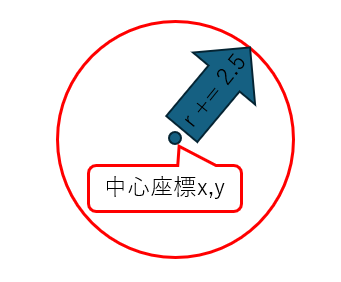
\includegraphics[width=6cm]{bomb_larger.png}
\end{center}
\caption{ボムは毎フレーム2.5ずつ拡大する}
\label{bomb_larger}
\end{minipage}
\begin{minipage}{0.5\hsize}
\begin{center}
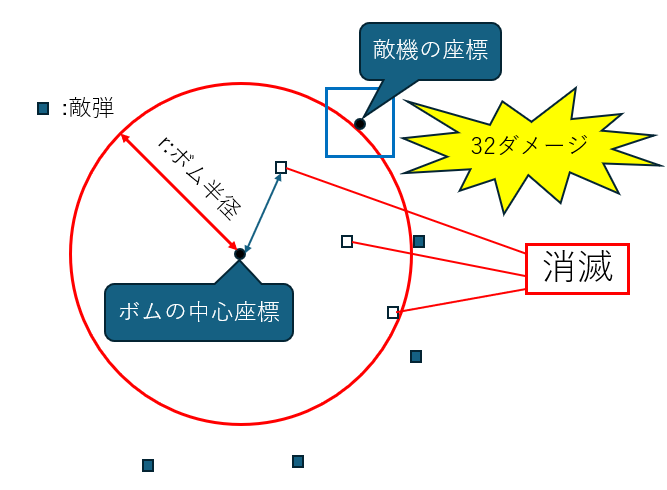
\includegraphics[width=6cm]{bomb_enemy.png}
\end{center}
\caption{ボムの敵・敵弾に対する処理}
\label{bomb_enemy}
\end{minipage}
\end{tabular}
\end{center}
\end{figure}
\subsection{敵機の動作}
\label{Enemy}
\subsubsection{敵機の基本動作}
\paragraph{使用した関数・変数}
敵機の基本動作の定義に使用した関数・変数は以下の表のとおり。
\begin{table}[H]
	\begin{center}
		\begin{tabular}{|c|c|c|}
			\hline
			型 & 変数・関数 & 説明\\  \hline \hline
			class & Enemy & 敵を定義するクラス \\ \hline
			float & x & 敵のx座標 \\ \hline 
			float & y & 敵のy座標 \\ \hline 
			float & xmove & 敵が向かうx位置 \\ \hline 
			float & ymove & 敵が向かうy位置 \\ \hline 
			float & HP & 敵のHP \\ \hline 
			bool & is\_boss & 敵機かどうか \\ \hline
			void & display() & 敵を表示する関数 \\ \hline 
			void & enemy\_move() & ランダムに敵を動かす関数 \\ \hline
			void & HP\_gauge() & 敵のHPゲージを表示する関数 \\ \hline 
			Enemy & enemy & 敵機を表すオブジェクト \\ \hline
			なし & murasame & 敵機の画像 \\ \hline
		\end{tabular}
	\end{center}
\end{table}
%敵のパラメータを書く
\paragraph{パラメータ}
以下に敵機の基本パラメータを記述する。
\begin{table}[H]
	\begin{center}
		\begin{tabular}{|c|c|}
			\hline
			パラメータ & 値\\ \hline \hline
			初期x座標 & 256 \\ \hline
			初期y座標 & 200 \\ \hline
			スピード & 5 \\ \hline
			最大HP & 16000 \\ \hline
			ボスかどうか & true \\ \hline
		\end{tabular}
	\end{center}
\end{table}
\paragraph{ソースコード}
以下のソースコードで敵機の動作処理を記述した。
\begin{lstlisting}
	void setup(){
		murasame = loadImage("murasame.png");
		enemy = new Enemy(Game_width / 2,height / 4,50,50,16000,16000,true);
    //Enemy(x初期値,y初期値,xサイズ,yサイズ,HP,Max_HP,ボスかどうか)
	}
void draw(){
		if (game_play && phase > 0) {
        enemy.display(); //敵を表示
        enemy.enemy_move(); //敵の動き
        enemy.HP_gauge(); //敵のHP
	}
}
	// 敵機のクラス
	class Enemy{
			//フィールドの宣言
			float x;
			float y;
			float xmove = Game_width / 2;
			float ymove = height / 4;
			float HP;
			float Max_HP;
			boolean is_boss;
			Enemy(float x, float y,float HP,float Max_HP, boolean is_boss) {
					this.x = x;
					this.y = y;
					this.HP = HP;
					this.Max_HP = Max_HP;
					this.is_boss = is_boss;
			}
			void display() {
					noStroke();
					image(murasame, x - 50, y - 45);
			}
			void enemy_move() {
					if (phase ==  1 && frameCount % 1000 == 0) {
							xmove = random(512);
							ymove = random(200);
					}
					else if (phase == 2 && frameCount % 500 == 0) {
							xmove = random(512);
							ymove = random(200);
					}
					else if (phase == 3 && frameCount % 200 == 0) {
							xmove = random(512);
							ymove = random(200);
					}
					else if (phase == 4 && frameCount % 300 == 0) {
							if (is_boss == false) {
									xmove = random(512);
									ymove = random(height);
							}
							if (is_boss == true && frameCount % 600 == 0) {
									xmove = random(512);
									ymove = random(400);
							}
					}
					if (!(x > xmove - 10 && x < xmove + 10)) {
							if (x < xmove) {
									x += 5;
							}
							else if (x > xmove) {
									x -= 5;		
							}
					}
					if (!(y > ymove - 10 && y < ymove + 10)) {
							if (y < ymove) {
									y += 5;
							}
							else if (y > ymove) {
									y -= 5;
							}
					}
			}
			void HP_gauge() {
					if (is_boss) {
							stroke(255);
							strokeWeight(3);
							line(0, 3, HP * (Game_width / Max_HP), 3);
					}
			}
	}
\end{lstlisting}
\paragraph{処理の説明}
%処理の説明を書く。
%xmove,ymoveを使って動作のメカニズムを説明。
ある一点をランダムに決める。するとその点を目指して敵が5ずつ動く。
目的店の四方10以内に敵が入ると敵は止まる。図\ref{random_move}
この際敵の動作を数式で表すと以下の通りになる。
\begin{gather*}
	敵機の座標を(x,y)、目的点の座標を(x',y')とすると、\\
	x = 
	\begin{cases}
		\begin{cases}
			x + 5 & (x < x') \\
			x - 5 & (x > x') \\
		\end{cases}
		& (x \geqq x' + 10),(x \leqq x' - 10) \\
		x & (x' -10 < x < x' + 10) \\
	\end{cases}
	\\
	y = 
	\begin{cases}
		\begin{cases}
			y + 5 & (y < y') \\
			y - 5 & (y > y') \\
		\end{cases}
		& (x \geqq y' + 10),(y \leqq y' - 10) \\
		y & (y' -10 < y < y' + 10) \\
	\end{cases}
\end{gather*}
\begin{figure}[H]
\begin{center}
\includegraphics*[height = 6cm]{random_move.png}
\caption{敵がランダムに動く原理}
\label{random_move}
\end{center}
\end{figure}
また初めは敵が目的点に到達したときに止まるように定義したが
\begin{itemize}
	\item スピードを1にすると目的点に到達するのが遅く位置が定まらない
	\item スピードを5にすると調整が難しく、位置が定まらない
\end{itemize}
という問題があったため範囲を設定した。
また各フェーズによって動作頻度は異なる。その表を以下に示す。
\begin{table}[H]
	\centering
	\begin{tabular}{|c|c|c|}
		\hline
		フェーズ & 移動頻度 & 移動範囲\\ \hline \hline
		1 & 1000フレーム & x座標:0~512 y座標 : 0~200\\ \hline
		2 & 500フレーム & 上に同じ\\ \hline
		3 & 200フレーム & 上に同じ\\ \hline
		4 & 300フレーム & x座標 : 0~512 y座標 : 0~800\\ \hline
	\end{tabular}
\end{table}
\subsubsection{フェーズ1}
フェーズ1では、プレイヤーはランダムに生成される$50 \times 50$平方の四角形を避けることになる。※図\ref{phase1}
\begin{figure}[H]
\begin{center}
\includegraphics*[height = 5cm]{phase1.png}
\caption{フェーズ1におけるゲーム画面}
\label{phase1}
\end{center}
\end{figure}
\paragraph{定義に使用した変数・関数}
新たに以下の変数・関数をフェーズ1の動作定義に使用した。
\begin{table}[H]
	\centering
	\begin{tabular}{|c|c|c|}
		\hline
		型・クラス & 変数・関数 & 説明 \\ \hline \hline
		ArrayList<Weapon> & Rect\_attack & 四角形を落とす必殺技のオブジェクト \\ \hline
		int & NumOfRect & 四角形の数 \\ \hline
		void & rect\_fall() & 四角形を落とす関数 \\ \hline
		void & control\_rect & 四角形の制御 \\ \hline
	\end{tabular}
\end{table}
\paragraph{パラメータ}
オブジェクトRect\_attackのパラメータを以下に示す。
\begin{table}[H]
	\centering
	\begin{tabular}{|c|c|}
		\hline
		パラメータ & 値 \\ \hline \hline
		初期x座標 & 0~500までのランダム値 \\ \hline
		初期y座標 & 0~200までのランダム値 \\ \hline
		弾速 & 10 \\ \hline
		攻撃力 & 15 \\ \hline
		発射頻度 & 10フレーム \\ \hline
		進行方向 & 下(y正方向) \\ \hline
	\end{tabular}
\end{table}

\paragraph{ソースコード}
フェーズ1の動作定義に使用したソースコードを以下に示す。
\begin{lstlisting}
void setup(){
	Rect_attack = new ArrayList<Weapon>(); //敵の玉を定義
}
void draw(){
	if(game_play && phase > 0){
		//第一フェーズの弾を生成
  	if (phase == 1 && frameCount % 10 == 0) {
  	  Rect_attack.add(new Weapon(random(500),random(200),10,15,0,0,0));
  	  NumOfRect++;
  	}
		control_rect();
	}	
}
class Weapon{
	//四角形を落とす
    void rect_fall() {
        noStroke();
        fill(x,y,400);
        y += speed;
        rect(x,y,50,50);
    }
}
void control_rect() {
    for (int i = 0; i < NumOfRect - 1; i++) {
        Rect_attack.get(i).rect_fall(); //四角形を落とす。
        if (NumOfRect > 1) {
            if (Rect_attack.get(i).y> height || Rect_attack.get(i).x > Game_width) {
                //四角形弾が画面外に出たとき。
                Rect_attack.remove(i); //四角形を削除
                NumOfRect--;
            }
            if ((Rect_attack.get(i).x < player.x + 25 && Rect_attack.get(i).x > player.x - 25) && (Rect_attack.get(i).y < player.y + 25 && Rect_attack.get(i).y > player.y - 25)) {
                //四角形がプレイヤーの当たり判定と衝突したとき
                player.HP -= Rect_attack.get(i).atk; //プレイヤーが四角形の攻撃力分だけダメージを受ける
                Rect_attack.remove(i); //四角形を削除する
                NumOfRect--; //四角形のカウントを減らす。
            }
        }
    }
}
\end{lstlisting}

\paragraph{処理の説明}
このフェーズでは以下のようにオブジェクトを処理する。
\begin{itemize}
	\item 四角形の色は、色相をx座標の値、彩度をy座標の値、明度を400としている。\ref{rect_fall}
	\item 画面外に出たもしくはプレイヤーに当たった時弾を削除する。
	\item 四角形は1フレームにつき10下に落ちる。※図\ref{rect_fall}
	\item プレイヤーの当たり判定は四方25である。※	図\ref{rect_attack}
	\item プレイヤーが四角形に当たった時プレイヤーは15ダメージを受ける。※図\ref{rect_attack}
\end{itemize}
%横に2枚の画像(jpg/png)表示
\begin{figure}[H]
\begin{center}
\begin{tabular}{c}
\begin{minipage}{0.5\hsize}
\begin{center}
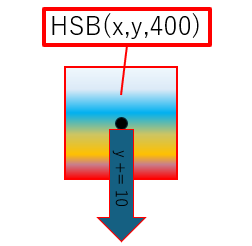
\includegraphics[width=6cm]{rect_fall.png}
\end{center}
\caption{rect\_fall()関数での処理}
\label{rect_fall}
\end{minipage}
\begin{minipage}{0.5\hsize}
\begin{center}
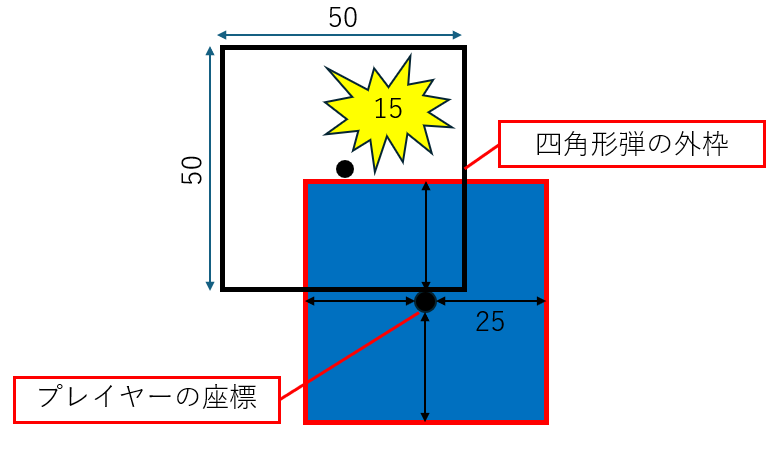
\includegraphics[width=10cm]{control_rect.png}
\end{center}
\caption{rect\_control()関数での処理}
\label{rect_attack}
\end{minipage}
\end{tabular}
\end{center}
\end{figure}
\subsubsection{フェーズ2}
フェーズ2ではプレイヤーは軌道をずらしながら発射される円状の攻撃弾を避けることになる。※図\ref{phase2_1}

また敵の中心座標から弾が発射されるため、敵が移動すると軌道が大きくずれる※図\ref{phase2_2}
%横に2枚の画像(jpg/png)表示
\begin{figure}[H]
\begin{center}
\begin{tabular}{c}
\begin{minipage}{0.5\hsize}
\begin{center}
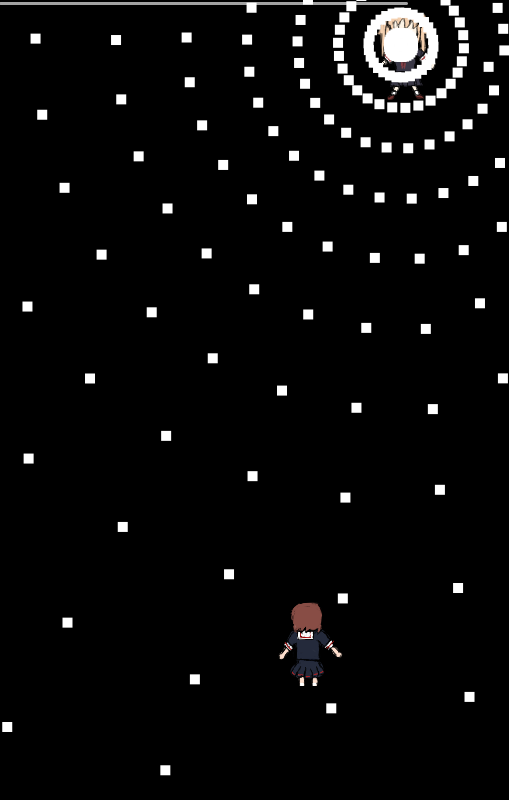
\includegraphics[width=5cm]{phase2_1.png}
\end{center}
\caption{通常時の弾幕}
\label{phase2_1}
\end{minipage}
\begin{minipage}{0.5\hsize}
\begin{center}
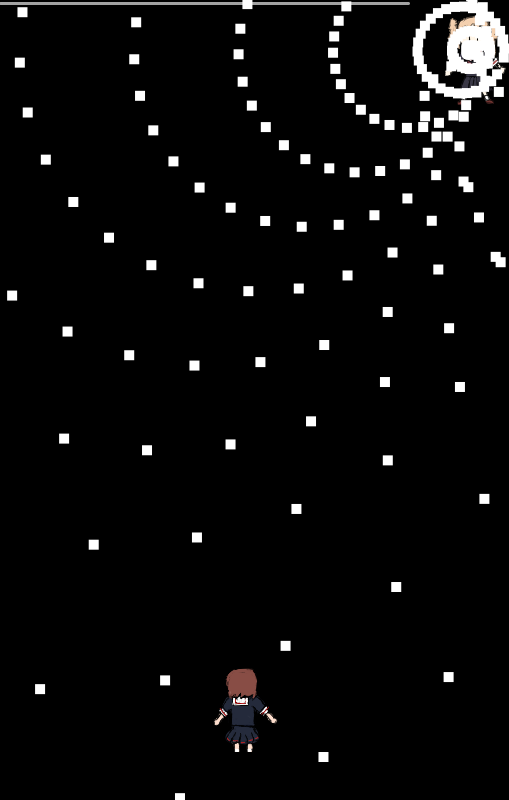
\includegraphics[width=5cm]{phase2_2.png}
\end{center}
\caption{敵が動いた時の弾幕}
\label{phase2_2}
\end{minipage}
\end{tabular}
\end{center}
\end{figure}

\paragraph{定義に使用した関数・変数}
以下の変数・関数をフェーズ2の動作定義に使用した。
\begin{table}[H]
	\centering
	\begin{tabular}{|c|c|c|}
		\hline
		型 & 変数・関数 & 説明\\ \hline \hline
		ArrayList<Weapon> & Cparts & 円状の攻撃弾を表すオブジェクト\\ \hline
		int & NumOfCParts & 攻撃弾の数\\ \hline
		float & vecX & 弾のxベクトル \\ \hline
		float & vecY & 弾のyベクトル \\ \hline
	\end{tabular}
\end{table}
\paragraph{パラメータ}
	オブジェクトCpartsのパラメータは以下の表のとおり。
	\begin{table}[H]
		\centering
		\begin{tabular}{|c|c|}
			\hline
			パラメータ & 値\\ \hline \hline
			x初期位置 & 敵機のx座標 \\ \hline
			y初期位置 & 敵機のy座標 \\ \hline
			弾速 & 3 \\ \hline
			攻撃力 & 5 \\ \hline
			発射頻度 & 10フレーム\\ \hline
			x進行方向(単位ベクトル) & (12 * (1~36の整数)) + (弾の数 / 30) \\ \hline
			y進行方向(単位ベクトル) & (12 * (1~36の整数)) + (弾の数 / 30) \\ \hline
		\end{tabular}
	\end{table}
\paragraph{ソースコード}
フェーズ2の動作定義に使用したソースコードを以下に示す。
\begin{lstlisting}
void setup(){
	Cparts = new ArrayList<Weapon>(); //敵の弾を定義
}
void draw(){
	if(game_play && phase > 0){
		//第二フェーズの弾を生成
		if (phase == 2 && frameCount % 10 == 0) {
				for (int i = 0; i < 30; i++) {
						//敵の中心から円状に弾を発射する。弾の数に応じて軌道を少しづつずらす。
						Cparts.add(new Weapon(enemy.x,enemy.y,3,5,0,(12 * i) + NumOfCParts / 30,(12 * i) + NumOfCParts / 30));
						NumOfCParts++;
				}
		}
		control_cparts();
		frameCount++;
	}
}
class Weapon{
	//円状に弾を発射する
	void cbullet() {
			noStroke();
			fill(0,0,400);
			r += speed / 30;
			x += r * vecX;
			y += r * vecY;
			rect(x,y,10,10);
	}
}
//円状弾の制御
void control_cparts() {
    if (NumOfCParts > 0) {
        for (int i = 0; i < NumOfCParts - 1; i++) {
            Cparts.get(i).cbullet(); //円形弾幕の操作。
            if (Cparts.get(i).y > height || Cparts.get(i).x > Game_width) {
                //弾が画面外に出たとき
                Cparts.remove(i); //弾を削除。
                NumOfCParts--;
            }
            if ((Cparts.get(i).x < player.x + 10 && Cparts.get(i).x > player.x - 10) && (Cparts.get(i).y < player.y + 10 && Cparts.get(i).y > player.y - 10)) {
                //プレイヤーに弾が当たった時(当たり判定サイズ:10)
                player.HP -= Cparts.get(i).atk; //プレイヤーがダメージを受ける
                Cparts.remove(i); //弾を削除する。
                NumOfCParts--; //弾のカウントを減らす。
            }
        }
    }
}
\end{lstlisting}
\paragraph{処理の説明}
フェーズ2では以下の処理を行う。※図\ref{Cparts}
\begin{enumerate}
	\item 12°感覚で弾を30個配置する。
	\item 弾と敵機の距離(発射半径)をスピード分大きくする。
	\item 発射角度を弾の数に応じてずらす。
	\item 1~3を繰り返す。
\end{enumerate}
座標定義を数式で表すと以下のようになる
\begin{gather*}
	弾の座標を(x,y)、敵機との距離をr、弾数をnとすると、\\
	x = r\cos(12 \times i + \frac{n}{30}) \\
	y = r\sin(12 \times i + \frac{n}{30}) \\
	また、フレーム更新時に、 \\ 
	r = r + 5\\ 
\end{gather*}

また当たり判定はプレイヤーの中心座標から四方10以内である。※図\ref{cb_attack}
%横に2枚の画像(jpg/png)表示
\begin{figure}[H]
\begin{center}
\begin{tabular}{c}
\begin{minipage}{0.5\hsize}
\begin{center}
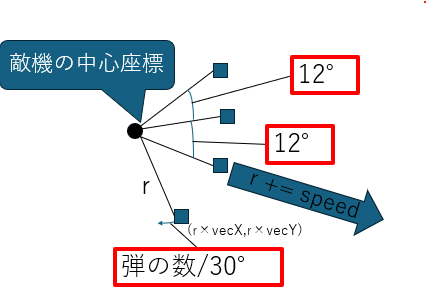
\includegraphics[width=6cm]{Cparts.png}
\end{center}
\caption{円状攻撃弾の発射原理}
\label{Cparts}
\end{minipage}
\begin{minipage}{0.5\hsize}
\begin{center}
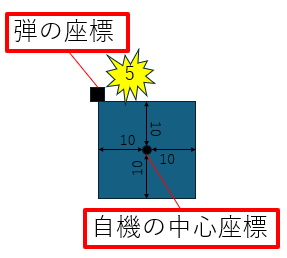
\includegraphics[width=4cm]{cb_attack.png}
\end{center}
\caption{円状攻撃弾の当たり判定}
\label{cb_attack}
\end{minipage}
\end{tabular}
\end{center}
\end{figure}
以上の処理で弾が座標をずらしながら円状に発射される必殺技を実装している。
\subsubsection{フェーズ3}
このフェーズでは、プレイヤーは上から降ってくるsinグラフの形に一定間隔で配置された弾(以降sin弾)と、
下から降ってくるcosグラフの形に一定間隔で配置された弾(以降cos弾)をよけることになる
※図\ref{phase3}
\begin{figure}[H]
\begin{center}
\includegraphics*[height = 8cm]{phase3_1.png}
\caption{フェーズ3におけるゲーム画面}
\label{phase3}
\end{center}
\end{figure}
\paragraph{使用した変数・関数}
フェーズ3の定義に使用した変数・関数は以下のとおりである。
\begin{table}[H]
	\centering
	\begin{tabular}{|c|c|c|}
		\hline
		型 & 変数・関数 & 説明 \\ \hline \hline
		ArrayList<Weapon> & sinb & sin弾を定義 \\ \hline
		ArrayList<Weapon> & cosb & cos弾を定義 \\ \hline
		float & A & sin,cos弾の振幅 \\ \hline
		float & fire & 一周期につき何個弾を並べるか \\ \hline
		float & T & 周期 \\ \hline
		float & biase & グラフをどれくらいずらすか。 \\ \hline
		int & NumOfsinb & sin弾の数 \\ \hline
		int & NumOfcosb & cos弾の数 \\ \hline
		void & tetrab() & sin,cos弾の表示、落下 \\ \hline
		void & control\_tetra() & sin,cos弾の制御 \\ \hline
	\end{tabular}
\end{table}
\paragraph{パラメータ}
sin,cos弾のパラメータを以下に示す。
\begin{table}[H]
	\centering
	\begin{tabular}{|c|c|c|}
		\hline 
		パラメータ & 値 & 対象 \\ \hline \hline
		T(周期) & 360 & 共通 \\ \hline
		fire(周期数) & 10 & 共通 \\ \hline
		A(振幅) & 50 & 共通 \\ \hline
		初期biase & 0 & 共通 \\ \hline
		i & 何周期目か & 共通 \\ \hline
		初期x座標 & $360 \times i + 36 \times (整数)$ & 共通 \\ \hline
		初期y座標 & $50\sin(36 * j)\circ$ & sin弾 \\ \hline
		初期y座標 & $50\cos(36 * j)\circ$ & cos弾 \\ \hline
		弾速 & 0.02 & 共通 \\ \hline
		攻撃力 & 5 & 共通 \\ \hline
		進行方向 & 下(y正方向) & sin弾 \\ \hline
		進行方向 & 上(y負方向) & cos弾 \\ \hline
	\end{tabular}
\end{table}
\paragraph{ソースコード}
フェーズ3の動作定義に使用したソースコードを以下に示す。
\begin{lstlisting}
void setup(){
	sinb = new ArrayList<Weapon>(); //sin弾を定義。
  cosb = new ArrayList<Weapon>(); //cos弾を定義。
}
void draw(){
	if(game_play && phase > 0){
		//第三フェーズの弾を生成。
		if (phase == 3 && frameCount % 60 == 0) {
				for (int i = 0; i < 2; i++) {
						for (int j = 0; j < T / fire; j++) {
								if (T * i + (T / fire) * j < Game_width) {
										//Sin状に弾を生成。
										sinb.add(new Weapon(T * i + (T / fire) * j , A * sin(radians(36 * j)),0.02,5,0,90,90));
										NumOfsinb++;
								}
								if (T * i + (T / fire) * j < Game_width) {
										//cos状に弾を生成
										cosb.add(new Weapon(T * i + (T / fire) * j , height - A * cos(radians(36 * j)),0.02,5,0,90, -90));
										NumOfcosb++;
								}
						}
				}
		}
		control_tetra();
		frameCount++;
	}
}
class Weapon{
	void tetrab() {
		x += biase * vecX;
		y += biase * vecY;
		noStroke();
		fill(0,0,400);
		rect(x,y,10,10);
		biase += speed;
	}
}
//sin弾の制御
void control_tetra() {
    if (NumOfsinb > 0) {
        for (int i = 0; i < NumOfsinb - 1; i++) {
            //各弾を動かす。
            sinb.get(i).tetrab();
            if (sinb.get(i).y > height) {
                //弾が画面外に出たとき
                sinb.remove(i); //sin弾を削除
                NumOfsinb--; //sin弾のカウントを減らす。
            }
            if ((sinb.get(i).x >= player.x - 10 && sinb.get(i).x <= player.x + 10) && (sinb.get(i).y >= player.y - 10 && sinb.get(i).y <= player.y + 10)) {
                //プレイヤーに弾が当たった時
                player.HP -= sinb.get(i).atk; //プレイヤーがダメージを受ける。
                sinb.remove(i); //sin弾を削除。
                NumOfsinb--; //sin弾のカウントを減らす。
            }
        }
    }
    if (NumOfcosb > 0) {
        for (int i = 0; i < NumOfcosb - 1; i++) {
            cosb.get(i).tetrab();  //各弾を動かす。
            if (cosb.get(i).y < 0) {
                //画面外に出たとき
                cosb.remove(i); //cos弾を削除
                NumOfcosb--; //cos弾のカウントを減らす。
            }
            if ((cosb.get(i).x >= player.x - 10 && cosb.get(i).x <= player.x + 10) && (cosb.get(i).y >= player.y - 10 && cosb.get(i).y <= player.y + 10)) {
                //プレイヤーに当たった時
                player.HP -= cosb.get(i).atk; //プレイヤーがダメージを受ける。
                cosb.remove(i); //cos弾を削除する。
                NumOfcosb--; //cos弾のカウントを減らす。
            }
        }
    }
}
\end{lstlisting}
\paragraph{処理の説明}
sin,cos弾の実装において、振幅、周期、一周期における弾数を定義し各弾のy座標にsin,cosを
かけている。バイアスの値を増やすことによって位置をずらし、降ってくる動きを実装している。
%横に2枚の画像(jpg/png)表示
\begin{figure}[H]
\begin{center}
\begin{tabular}{c}
\begin{minipage}{0.5\hsize}
\begin{center}
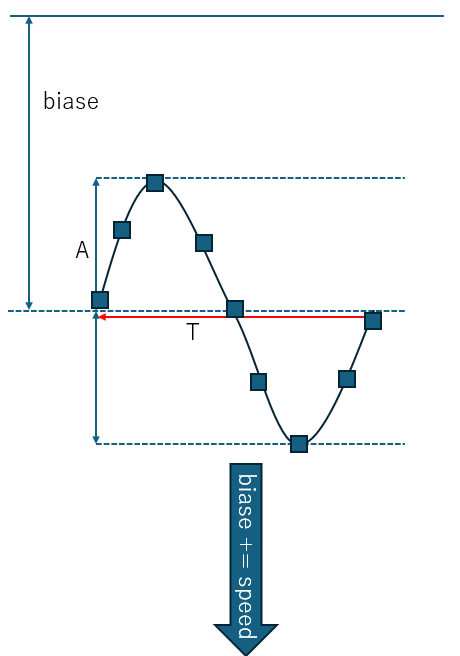
\includegraphics[width=3cm]{sinb.png}
\end{center}
\caption{sin弾の動く仕組み}
\label{}
\end{minipage}
\begin{minipage}{0.5\hsize}
\begin{center}
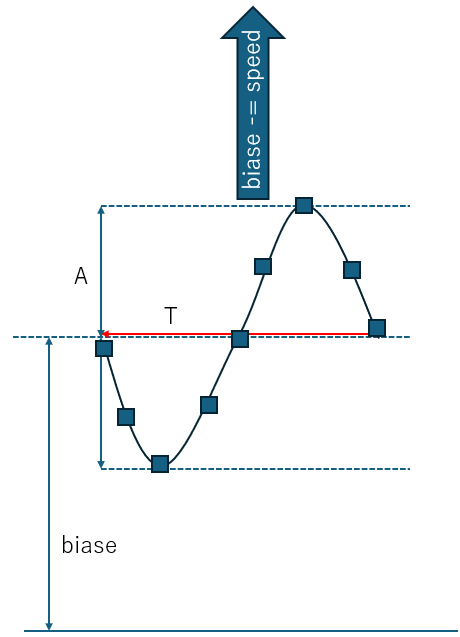
\includegraphics[width=3cm]{cosb.png}
\end{center}
\caption{cos弾の動く仕組み}
\label{}
\end{minipage}
\end{tabular}
\end{center}
\end{figure}
当たり判定の定義はフェーズ2の弾※図\ref{cb_attack}と同様である。
\subsubsection{フェーズ4}
フェーズ4では敵機が歯車型の敵を召喚し、歯車型の敵はランダムに動きながら
プレイヤーに向けて弾を打つ。それをよけながら敵を倒せばゲームクリアとなる。図\ref{phase4}
\begin{figure}[H]
\begin{center}
\includegraphics*[height = 8cm]{drawing_21.png}
\caption{フェーズ4におけるゲーム画面}
\label{phase4}
\end{center}
\end{figure}
\paragraph{使用した関数・変数}
フェーズ4の動作定義に新たに用いた関数・変数は以下のとおりである。
\begin{table}[H]
	\begin{tabular}{|c|c|c|}
		\hline
		型・クラス & 関数・変数 & 説明 \\ \hline \hline
		ArrayList<Enemy> & gear & 歯車型の敵を定義するオブジェクト \\ \hline
		ArrayList<Weapon> & gear\_bullet & 歯車の発射弾を定義するオブジェクト \\ \hline
		boolean & gear\_push & 歯車を発射したかどうか  \\ \hline
		int & NumOfgear & 歯車の数。初期値は8 \\ \hline
		int & NumOfgearb & 歯車の発射弾の数。 \\ \hline
		void & control\_gear() & 歯車型の敵を制御  \\ \hline
		void & gear() & 歯車型の敵を表示。 \\ \hline
		float & atan2() & 二点間の角度を求める関数。 \\ \hline
	\end{tabular}
\end{table}
\paragraph{パラメータ}
以下に歯車型の敵及びその発射弾のパラメータを示す。
\begin{table}[H]
  \begin{minipage}[h]{.45\textwidth}
    \begin{center}
      \begin{tabular}{|c|c|}
				\hline
				初期位置 & 敵機の座標 \\ \hline
				動作範囲 & x座標:0~512 y座標:0~800 \\ \hline
				移動頻度 & 300フレーム毎 \\ \hline
				スピード & 10 \\ \hline
				攻撃力 & 5 \\ \hline
				最大HP & 500 \\ \hline
				ボスかどうか & false \\ \hline
      \end{tabular}
    \end{center}
    \caption{歯車のステータス}
    \label{}
  \end{minipage}
  %
  \hfill
  %
  \begin{minipage}[h]{.45\textwidth}
    \begin{center}
      \begin{tabular}{|c|c|}
				\hline
				初期位置 & 歯車の座標 \\ \hline
				弾速 & 15 \\ \hline
				攻撃力 & 5 \\ \hline
				発射頻度 & 10 \\ \hline
				進行方向 & プレイヤーの方向  \\ \hline 
      \end{tabular}
    \end{center}
    \caption{歯車の弾のパラメータ}
    \label{}
  \end{minipage}
\end{table}

\paragraph{ソースコード}
フェーズ4の動作定義に使用したソースコードを以下に示す。
\begin{lstlisting}
void setup(){
	gear = new ArrayList<Enemy>(); //歯車型の敵を定義
	gear_bullet = new ArrayList<Weapon>(); //ギアの発射弾を定義。
}
void draw(){
	if(game_play && phase > 0){
		//第四フェーズの要素を生成。
		if (phase == 4) {
				if (gear_push) {
						NumOfgear = 8;
						for (int i = 0; i < NumOfgear; i++) {
								//歯車を生成。
								gear.add(new Enemy(enemy.x,enemy.y,50,50,5000,5000,false));
						}
						gear_push = false;
				}
				if (frameCount % 10 == 0) {
						float dx,dy;
						for (int i = 0; i < NumOfgear - 1; i++) {
								//プレイヤーと歯車の間の距離を算出
								dx = player.x - gear.get(i).x;
								dy = player.y - gear.get(i).y;
								//歯車の中心からプレイヤーの方向に進む弾を生成。
								gear_bullet.add(new Weapon(gear.get(i).x,gear.get(i).y,10,5,0,degrees(atan2(dy,dx)),degrees(atan2(dy,dx))));
								//歯車の弾をカウント。
								NumOfgearb++;
						}
						//プレイヤーと敵の間の距離を算出。
						dx = player.x - enemy.x;
						dy = player.y - enemy.y;
						//敵が発射する玉を歯車の弾の一部として扱う。歯車の弾よりも早い速度で発射する。
						gear_bullet.add(new Weapon(enemy.x,enemy.y,15,5,0,degrees(atan2(dy,dx)),degrees(atan2(dy,dx))));
						//ギアの弾の数を増やす。
						NumOfgearb++;
				}
		}
	}
}
class Enemy{
	//歯車を描画。
    void gear() {
        noStroke();
        fill(400,400,400);
        ellipse(x,y,50,50);
        for (int i = 0; i < NumOfgear; i++) {
            pushMatrix();
            fill(0);
            translate(x,y);
            rotate(radians(5 * frameCount));
            rect(0,0,10,10);
            translate(30 * cos(radians((360 * i / 8))),30 * sin(radians(360 * i / 8)));
            rotate(radians(360 * i / 8));
            noStroke();
            fill(400,400,400);
            rect( -1, -1,10,10);
            popMatrix();
        }
    }
}
//ギア(歯車)の制御。
void control_gear() {
    for (int i = 0; i < NumOfgear - 1; i++) {
        gear.get(i).gear(); //歯車を描画。
        gear.get(i).enemy_move(); //歯車を動かす。
        for (int j = 0; j < NumOfBullet - 1; j++) {
            if (dist(bullets.get(j).x,bullets.get(j).y,gear.get(i).x,gear.get(i).y) < 30) {
                //歯車の当たり判定に自機弾が当たった時
                gear.get(i).HP -= bullets.get(j).atk; //歯車が自機弾の攻撃力分だけダメージを受ける
                bullets.remove(j); //自機弾を消去
                NumOfBullet--; //弾の数のカウントを減らす。
            }
        }
        for (int j = 0; j < NumOfBullet2 - 1; j++) {
            if (dist(bullet2.get(j).x,bullet2.get(j).y,gear.get(i).x,gear.get(i).y) < 30) {
                //自機弾(二個目)が歯車に当たった時
                gear.get(i).HP -= bullet2.get(j).atk; //歯車のHP
                bullet2.remove(j); //自機弾(二個目)を削除する。
                NumOfBullet2--; //自機弾(二個目)のカウントを減らす。
            }
        }
        if (gear.get(i).HP < 0) {
            //ギアのHPが0を下回ったとき
            gear.remove(i); //ギアを消す。
            NumOfgear--; //ギアの数を減らす。
        }
    }
    for (int i = 0; i < NumOfgearb - 1; i++) {
        gear_bullet.get(i).cbullet(); //ギアの発射弾を動かす。
        if ((gear_bullet.get(i).x < player.x + 25 && gear_bullet.get(i).x > player.x - 25) && (gear_bullet.get(i).y <player.y + 25 && gear_bullet.get(i).y > player.y - 25)) {
            //ギアの発射弾がプレイヤーに当たった時。
            player.HP -= gear_bullet.get(i).atk; //プレイヤーがダメージを受ける。
            gear_bullet.remove(i); //ギアの発射弾を削除する。
            NumOfgearb--; //ギアの発射弾のカウントを減らす。
        }
        if (gear_bullet.get(i).y > height || gear_bullet.get(i).y < 0 || gear_bullet.get(i).x > Game_width) {
            //ギア弾が画面外に出たとき
            gear_bullet.remove(i); //ギア弾の削除
            NumOfgearb--; //ギア弾のカウントを減らす。
        }
    }
}
\end{lstlisting}
\paragraph{処理の説明}
歯車の描画から先に説明する。
歯車は二重円を描画しそこに四角形を付け加えることで実現している。
また付け加えた四角形を回転させながら二重円の周りを回らせることで歯車が回転する演出を
実現している。※図\ref{gear}

基本的な歯車の挙動は敵機の挙動に準拠する。

プレイヤーに向かって弾を発射する挙動についてはatan2関数でプレイヤーと歯車との間の
角度を求めてそれを基に発射方向を定めるといった処理を行っている。※図\ref{atan2}

%横に2枚の画像(jpg/png)表示
\begin{figure}[H]
\begin{center}
\begin{tabular}{c}
\begin{minipage}{0.5\hsize}
\begin{center}
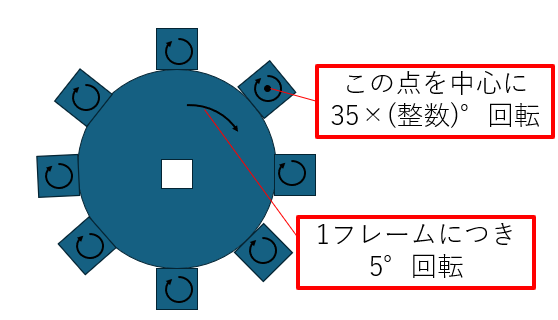
\includegraphics[width=8cm]{gear.png}
\end{center}
\caption{歯車の描画}
\label{gear}
\end{minipage}
\begin{minipage}{0.5\hsize}
\begin{center}
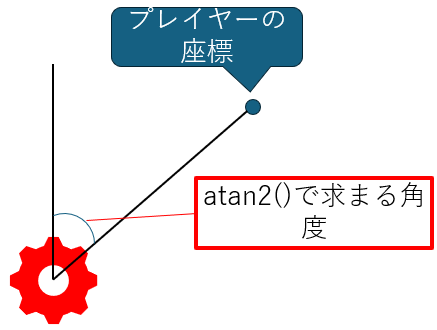
\includegraphics[width=8cm]{atan2.png}
\end{center}
\caption{歯車の弾の制御}
\label{atan2}
\end{minipage}
\end{tabular}
\end{center}
\end{figure}



歯車の弾の当たり判定はプレイヤーの四方25である。

歯車本体の当たり判定は半径30以内である。
\section{結果と考察}
以上のアプリを制作した結果、学科内ランキング9位という結果であった。
\subsection{他者からの評価とそれに対する考察}
以下のような他者からの評価が見られた。
\begin{itemize}
	\item きちんと東方になっていた
	\item ゲームバランスが良かった
	\item 弾幕が手が込んでいてよかった。
	\item 複数の攻撃手段があり面白かった
	\item 弾幕に画面酔いしてしまった
\end{itemize}
\subsection{問題点とその解決法}
弾幕に画面酔いする問題については改善しなければならない。
フェーズ2,3,4共に弾幕を白い四角形にしたため視認性が悪く画面酔いをしてしまったと思われる。
この点については視認性の良いグラフィックを制作することで改善できる。

そしてその次はコードの視認性の悪さである。現在操作しているオブジェクトを
指し示す「this」や、引数を活用すればもっと短く整理されたコードで記述できたのではないかと考えている。
\section{まとめ}
当初の目的であった知っているシューティングゲームの挙動を一通り実装できるようになるという目的に
ついては、基本的なものでさえ参考にした東方の挙動を実現するのは難しかったためこれは実現できなかった
ということになる。

ゲーム制作の基礎を体感しゲームプログラミングの基礎を理解することについては達成できた。
ゲームの作り始め方すら知らなかった段階からこのゲームが作れたことは誇るべきことだろう。

ゲームクリエイターの独創性を理解することについては少し達成出来た。東方原作者のZUN氏の
凄みを微量ながら知った。

本実験の目的である新しい開発プラットフォームを使いこなせるようにする学習能力を身に着けること
についてはいい経験になった。現にいまJavascriptのプラグインThree.jsやOPEN GL等のツールに
抵抗なく触れることができている。
\subsection{感想}
今回のゲーム制作及びレポート執筆を終えてわかったことは、一連のプログラムを
作って極力わかりやすいように報告書を作ることはかなりの労力を要する
難しい作業なのだということである。表や画像を極力用いたがそれでも自分の意図が
伝わってくれという気持ちである。加えて説明に36ページも要した。もっと簡潔に短く
書くべきだったと後悔している。しかし今回の講義は自分を一番成長させる有意義な
講義であった。
\end{document}
\begin{itemize}